% Ubah judul dan label berikut sesuai dengan yang diinginkan.
% \section{Architecture}
% \label{sec:architecture}

% Update the title and label below as desired.
\section{Design and Implementation}
\label{sec:designandimplementation}

This research will 

\begin{figure}[ht]
  \centering
  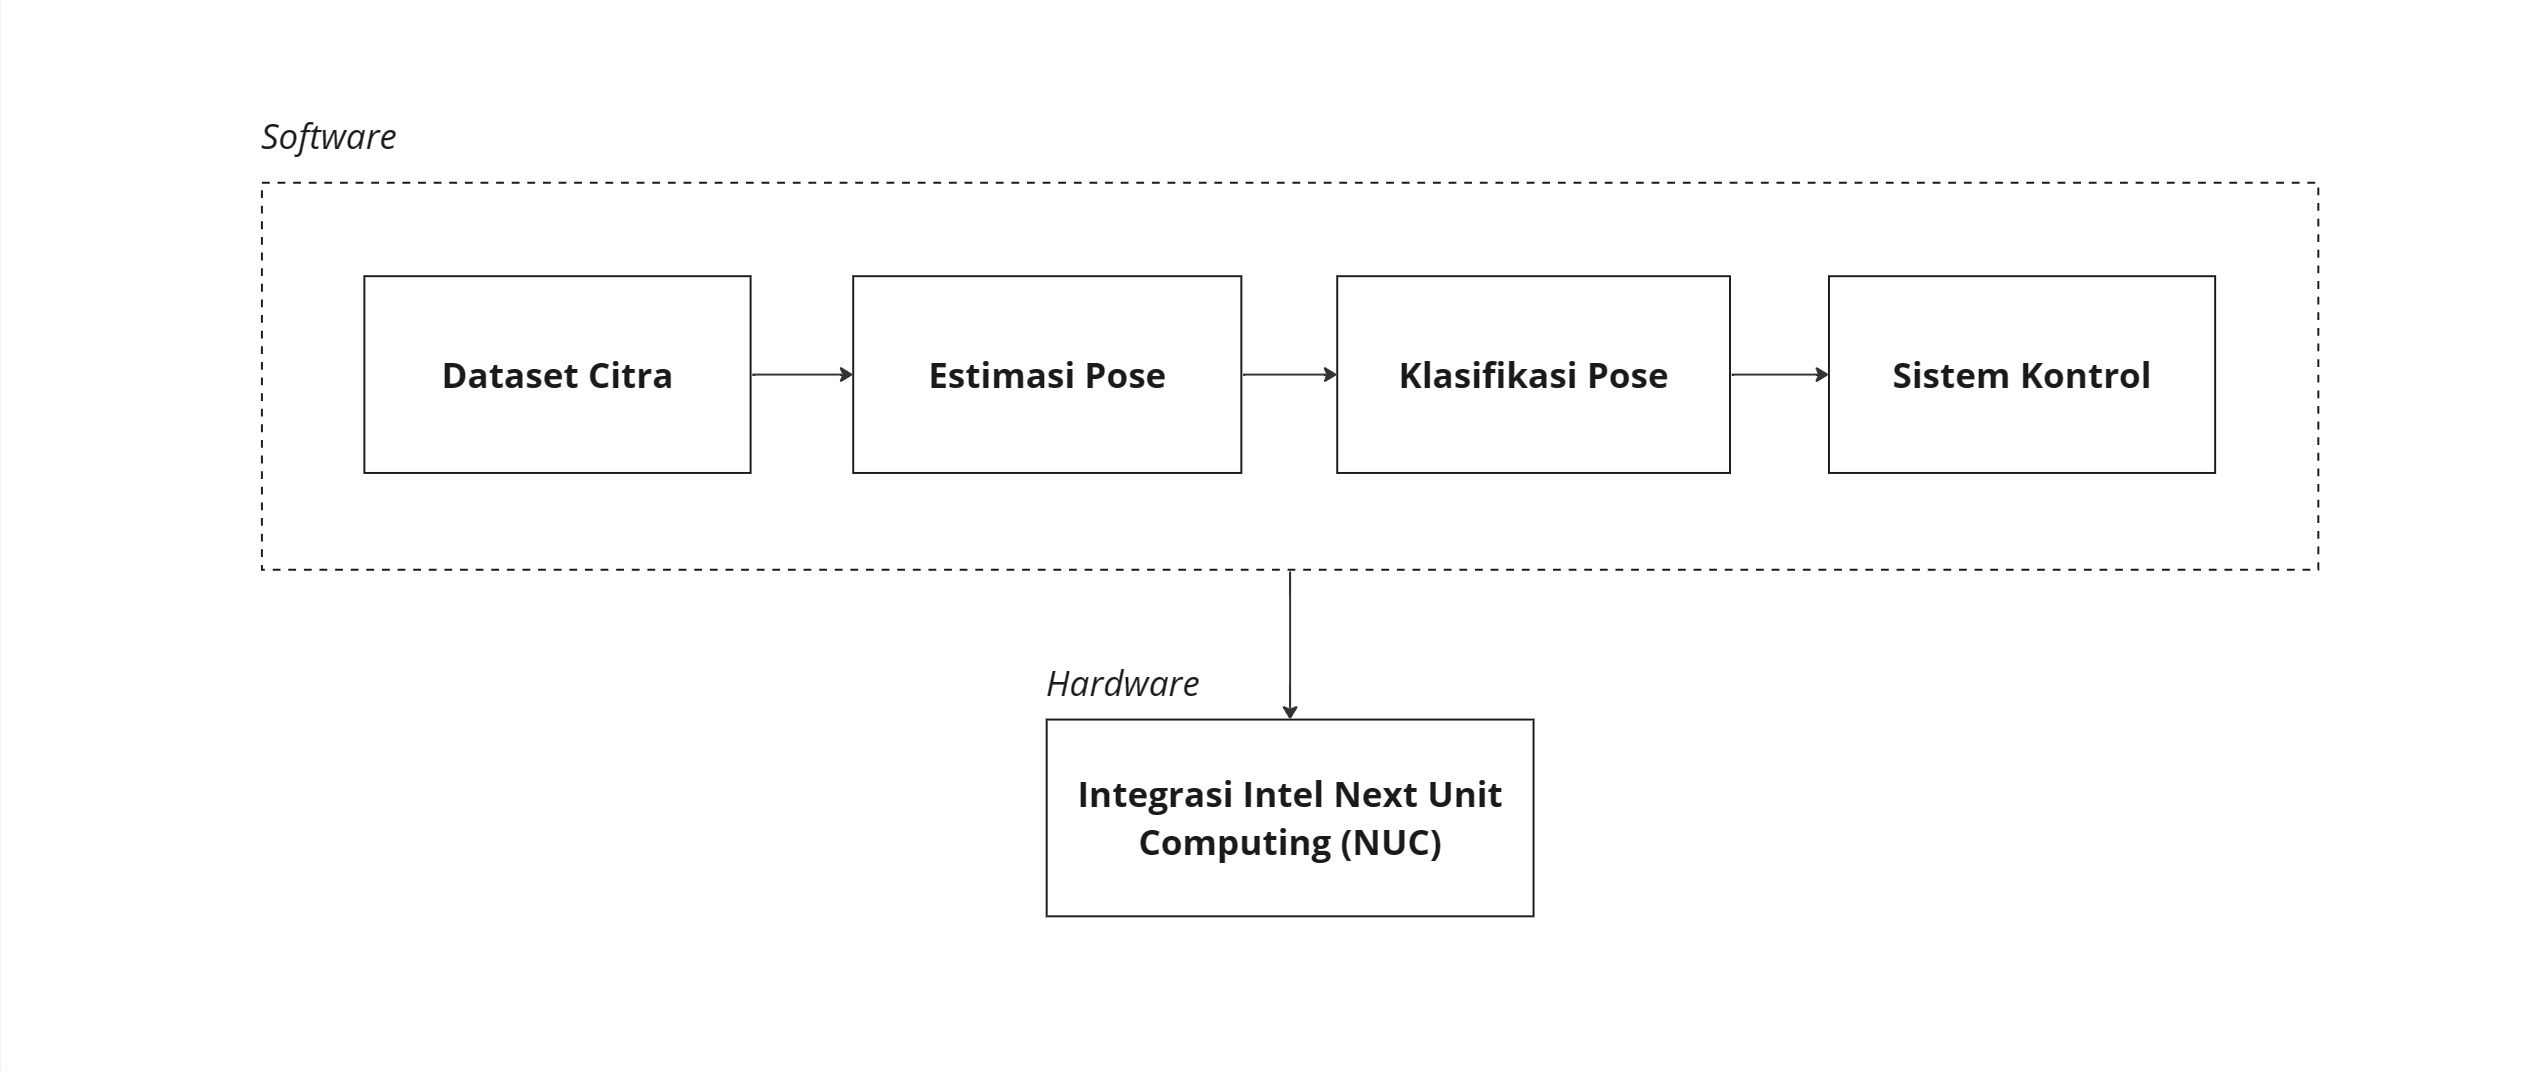
\includegraphics[scale=0.1]{gambar/bab3-block-diagram-nuc.jpg}
  \caption{Research flow}
  \label{fig:blockdiagrammethod}
\end{figure}

\subsection{Image Dataset}
\label{subsec:imagedataset}

The dataset used is a collection of images measuring 640 pixels x 480 pixels. The image data is obtained using the OpenCV library to capture video, which is then extracted into 30 frames for each data. Six BISINDO vocabulary signs with general vocabulary context and three control signs are used to facilitate system use. In sequence, the control vocabulary "standby" (indicates vocabulary transition), "delete" (deletes vocabulary), and "translate" (converts to voice).

\begin{table}[H]
  \caption{BISINDO and Control Vocabulary}
  \label{tb:kosakataBISINDO}
  \centering
  \begin{tabular}{lll}
    \toprule
    \textbf{Class} & \textbf{Data Count} & \textbf{Frame Count} \\
    \midrule
    Sorry                       & 30            & 30 \\
    Please                      & 30            & 30 \\
    I                           & 30            & 30 \\
    Name                        & 30            & 30 \\
    Home                        & 30            & 30 \\
    Who                         & 30            & 30 \\
    \textit{Standby}                       & 30             & 30 \\
    \textit{Translate}                     & 30             & 30 \\
    \textit{Delete}                        & 30             & 30 \\
    \bottomrule
  \end{tabular}
\end{table}

\subsection{Pose Estimation}
\label{subsec:poseestimation}

\begin{figure}[ht]
  \centering
  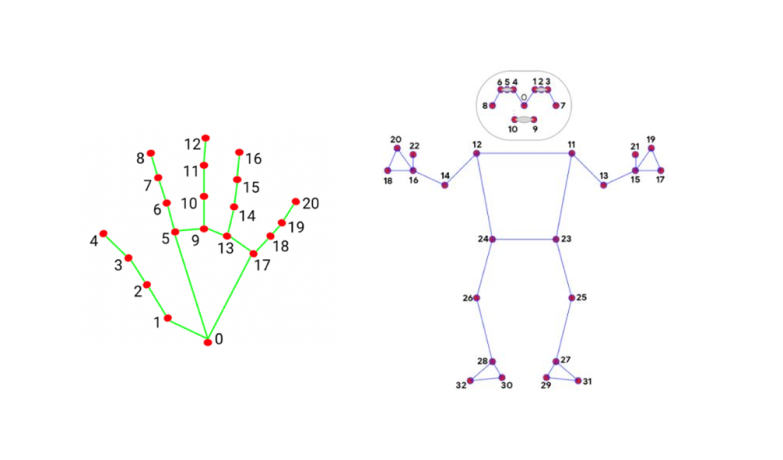
\includegraphics[scale=0.4]{gambar/bab3-pose-combine.png}
  \caption{Mediapipe Pose and Hand}
  \label{fig:estimasipose}
\end{figure}

For each image in the 30 data, pose estimation was performed with the help of the MediaPipe framework. In the formation of BISINDO signs, the moving parts of the body are the hands and arms. Through MediaPipe hand, 21 landmarks are extracted from the hand, so the total landmarks for the right and left hands are 42 landmarks. In MediaPipe pose, landmarks from the shoulder to the arm will be extracted, so the landmarks used will only be in positions 11 to 22, giving a total of 12 landmarks for the body. For each landmark, the x and y coordinates are obtained. This data is then normalized to produce a scale-invariant model (adaptable to the user's shape) and position-invariant (adaptable to the user's position). The following are the normalization formulas to be used:

\begin{equation}
  \label{eq:shouderWidthNorm}
  w = \sqrt{(x_{ka} - x_{ki})^2 + (y_{ka} - y_{ki})^2}
\end{equation}
\vspace{5mm}
\begin{equation}
  \label{eq:shoulderMidpointNorm}
  x_m = \frac{x_{ka} + x_{ki}}{2} ; \\
   y_m = \frac{y_{ka} + y_{ki}}{2}
\end{equation}
\vspace{5mm}
\begin{equation}
  \label{eq:normalization}
  x'_i = \frac{x_i - x_m}{w} ;  \\
   y'_i = \frac{y_i - y_m}{w}
\end{equation}

\subsection{Pose Classification}
\label{subsec:poseclassification}

The LSTM model used has a sequential architecture to combine a series of layers to produce a high-performing sign language translation model. The first layer is a TimeDistributed layer with a Dense layer of 128 units, 'tanh' activation, and an input shape of (30, 108), where each frame is processed independently with consistent Dense layers for each frame. The second layer is the first LSTM with 128 units, return\_sequences=True, 'tanh' activation, and an input shape of (30, 108). The third layer is a Dropout layer with a value of 0.5 to prevent excessively high weights. The fourth layer is the second LSTM with 128 units, return\_sequences=False, and 'tanh' activation, followed by a Dropout layer with a value of 0.5. To simplify the complexity of the output data from the two LSTM layers, a Dense layer with 128 units and 'relu' activation is used, followed by a Dropout layer with a value of 0.2 to prevent overfitting. The final layer is a Dense layer with 'softmax' activation and the number of units according to the number of categories. This model is compiled using the Adam optimizer and categorical crossentropy as the loss function, with categorical accuracy metrics to monitor performance during training.

\subsection{Control System}
\label{subsec:controlsystem}

The control system is a series of processes that will regulate how sign language will be detected, handle detection errors, combine various words into sentences, delete vocabulary, and translate sentences into voice. This control system is expected to facilitate the use of the translator system. The control system will be divided into two: the sign language detection program and the sentence formation program.

\newpage

\begin{figure}[H]
  \centering
  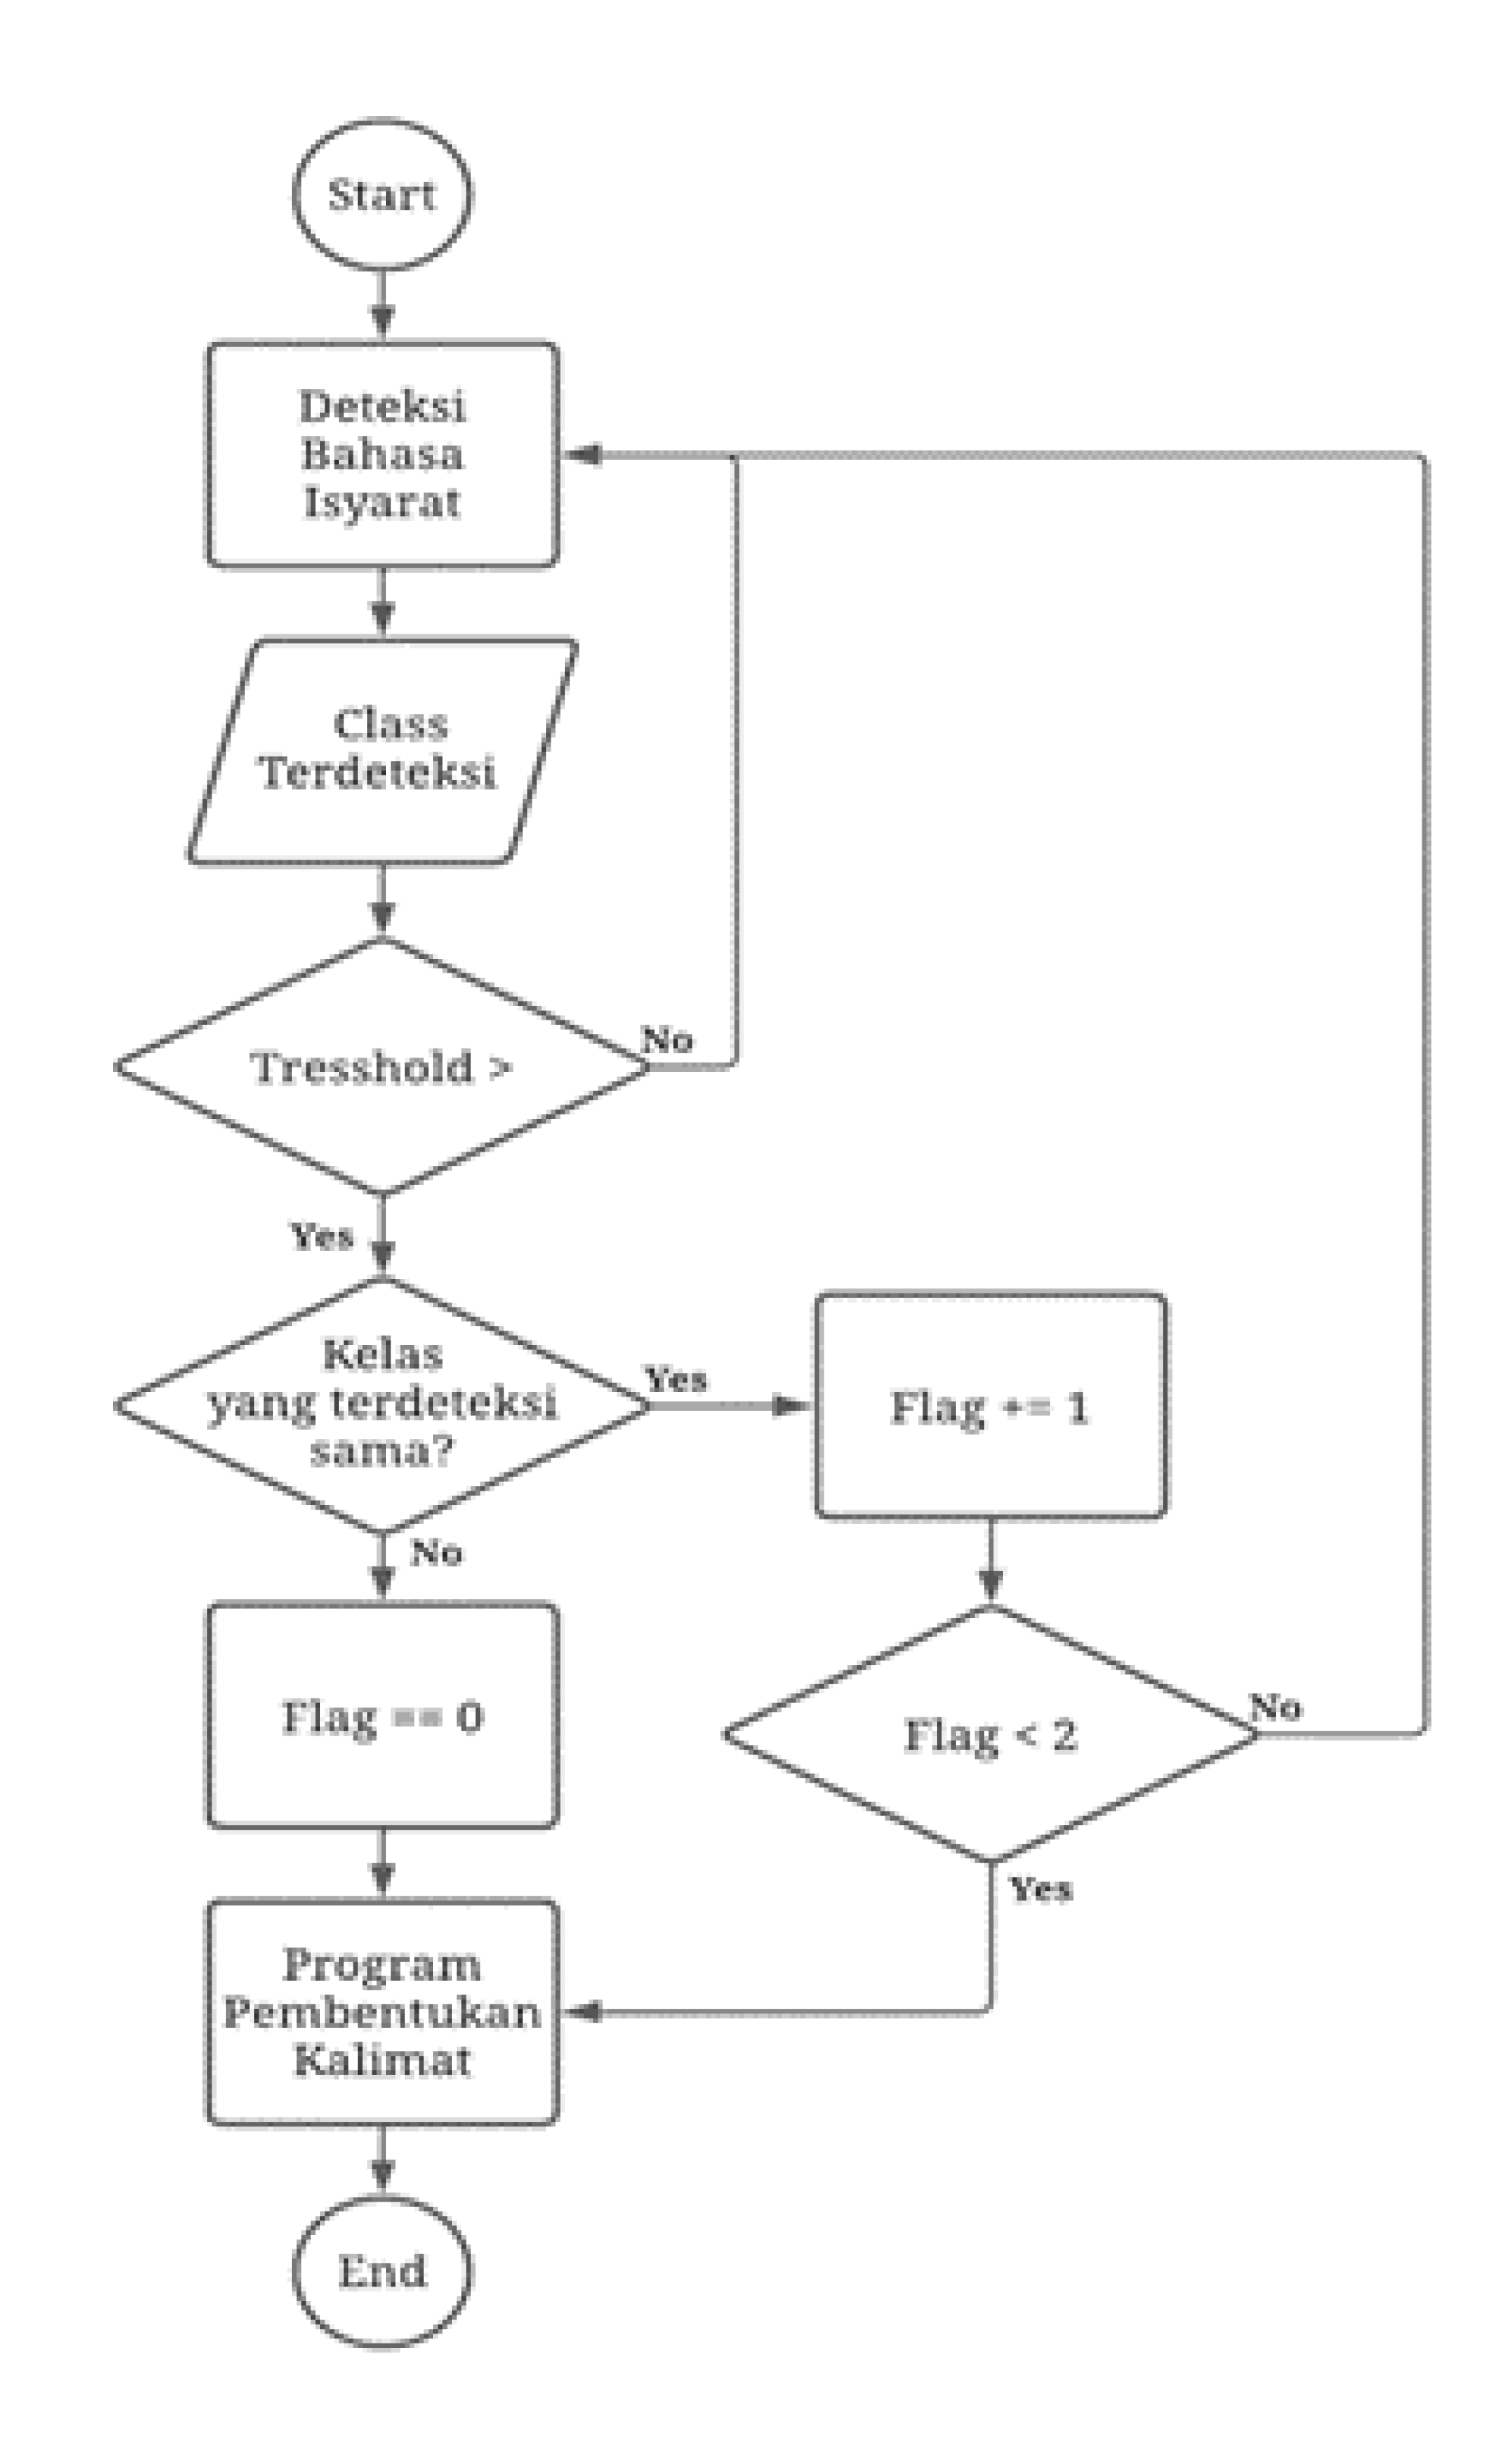
\includegraphics[scale=0.37]{gambar/bab3-flowchart-deteksi.png}
  \caption{Sign language detection program flowchart}
  \label{fig:flowchartdeteksi}
\end{figure}

\begin{figure}[H]
  \centering
  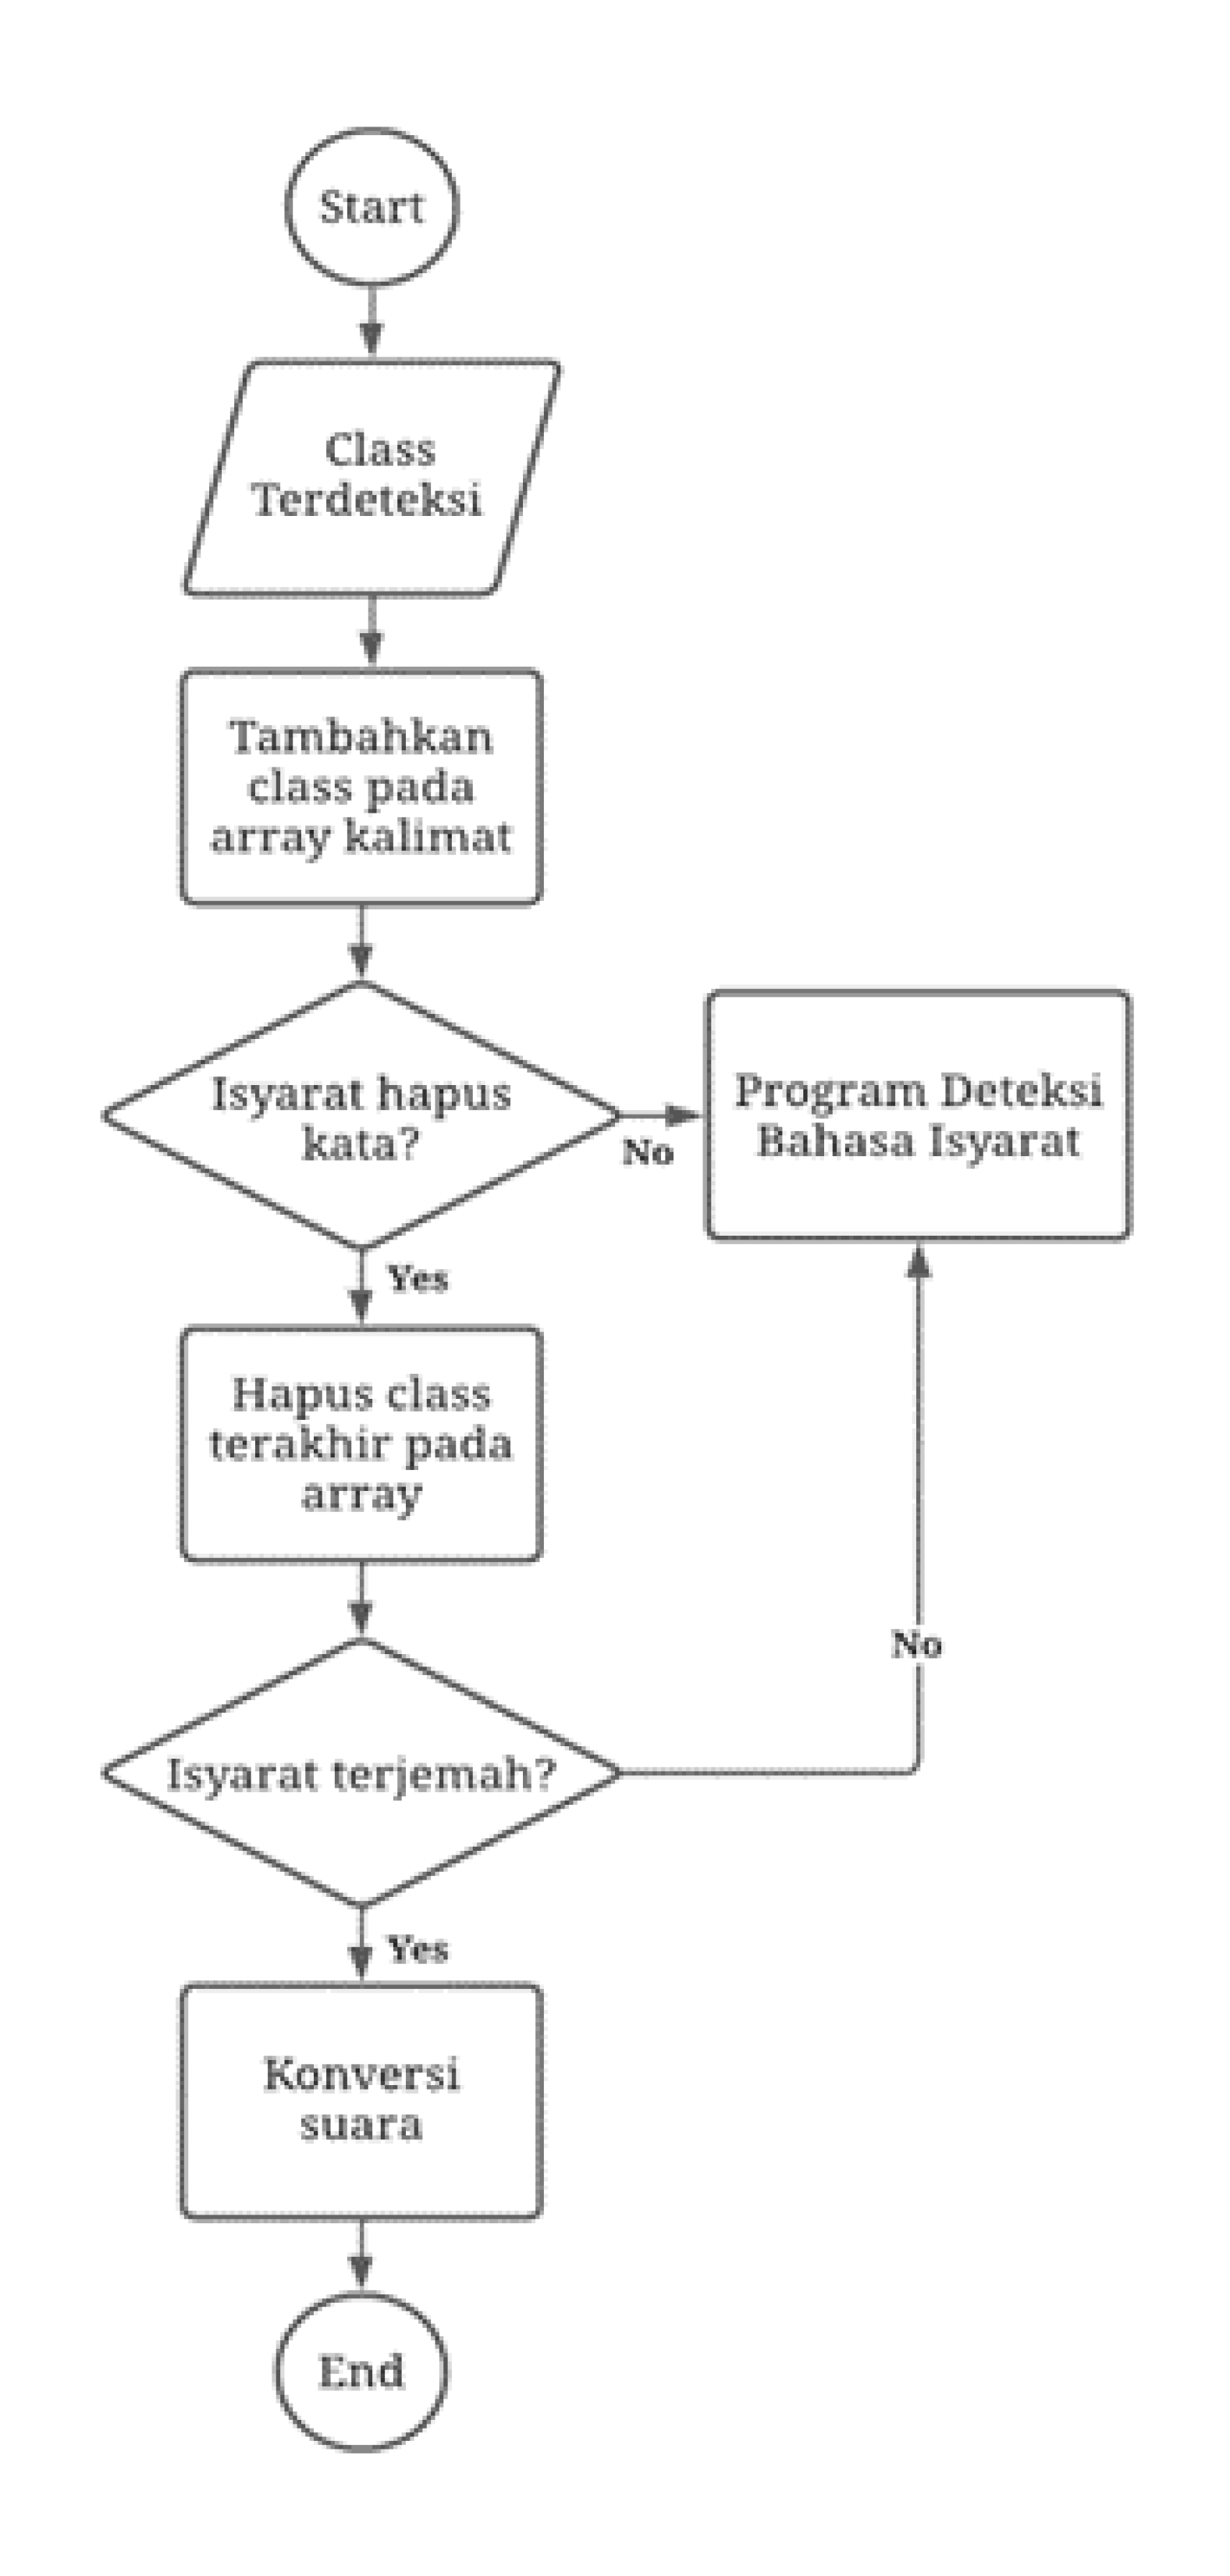
\includegraphics[scale=0.37]{gambar/bab3-flowchart-kalimat.png}
  \caption{Sentence formation program flowchart}
  \label{fig:flowchartkalimat}
\end{figure}

\subsection{Integration of \emph{Next Unit Computing} (NUC)}
\label{subsec:integrasiNUC}

Integration with Intel NUC is done by accessing a website created using the Streamlit framework, which is connected to a computer server via port forwarding. The website will access the user's webcam, allowing them to perform sign movements, which are then classified with the previously trained LSTM model in real-time.



% % Ubah paragraf-paragraf pada bagian ini sesuai dengan yang diinginkan.

% \subsection{Cetak Biru Roket}
% \label{subsec:cetakbiruroket}

% Pada cetak biru yang tertera pada Gambar \ref{fig:cetakbiru}. \lipsum[8]

% % Contoh input gambar pada kolom.
% \begin{figure} [ht]
%   \centering
%   % Ubah sesuai dengan nama file gambar dan ukuran yang akan digunakan.
%   \includegraphics[width=0.4\textwidth]{gambar/cetakbiru.jpg}

%   % Ubah sesuai dengan keterangan gambar yang diinginkan.
%   \caption{Cetak biru roket yang akan diuji coba. \cite{cetakbiruspacex}}
%   \label{fig:cetakbiru}
% \end{figure}

% \lipsum[9-10]

% \subsection{Lorem Ipsum}
% \label{subsec:loremipsum}

% \lipsum[11]

% % Contoh pembuatan tabel.
% \begin{table}
%   \caption{Contoh tabel sederhana}
%   \label{tab:tabelsederhana}
%   \centering
%   \begin{tabular}{lll}
%     \toprule
%     Heading1 & Heading2 & Heading3 \\
%     \midrule
%     One      & Two      & Three    \\
%     Four     & Five     & Six      \\
%     \bottomrule
%   \end{tabular}
% \end{table}

% % Contoh pembuatan potongan kode.
% \begin{lstlisting}[
%   language=C++,
%   caption={Program halo dunia.},
%   label={lst:halodunia}
% ]
% #include <iostream>

% int main() {
%     std::cout << "Halo Dunia!";
%     return 0;
% }
% \end{lstlisting}

% \lipsum[12]

% % Contoh pembuatan daftar.
% \begin{enumerate}
%   \item \lipsum[13][1-4]
%   \item \lipsum[13][5-8]
%   \item \lipsum[13][9-12]
% \end{enumerate}

% \lipsum[14-15]
